\chapter{Полунатурное моделирование}
\label{ss:hw}

Задачей полунатурного эксперимента являлась верификации возможности применения предлагаемого подхода к оценке параметров сигнала СПИ с ШПС. Для определения наличия источников
сигнала был применен классический параллельный коррелятор \cite{tsui} с шагом по частоте 1 кГц и диапазоном 5 кГц. Данный диапазон обусловлен максимальным Допплеровским
смещением частоты для стационарного приемника в СПИ Navstar GPS \cite{shahtarin_sync, tsui}. 

\section{Аппаратная платформа}
Представленная аппаратная платформа была разработана автором в процессе дипломного проектирования в Московском Государственном Университете Приборостроения и Информатики (МГУПИ).

Данная аппаратная платформа предоставляет пользователю возможность получать необработанный сигнал со спутников СНС Navstar GNSS. В текущей реализации поддерживается только 
СНС Navstar GPS, однако чип так же может принимать сигналы СНС Galileo и СНС Глонасс. Дампы данных представляют собой текстовые файлы. В них содержится 256 КБ необработанных данных.
На частоте оцифровки 256 КБ представляет чуть более 6 мс данных. Данного объема хватает для оценки параметров источников сигналов СНС Navstar GPS.
В данный момент аппаратная платформа используется как лабораторный стенд в МГУПИ по курсу ЦОС. Платформа позволяет работать с реальным сигналом, что является большим плюсом в
виду того, что позволяет наглядно продемонстрировать работу алгоритмов обработки сигнала, а так же проверить теоретические предположения в реальных условиях.
Так же на базе платы разрабатывается ряд дипломных работ в области СНС систем (например создание аппаратного коррелятора на VHDL или создание модели канала 
СПИ Navstar GPS данных). Исходники прошивки платы расположены в публично доступном хранилище кода github.com \cite{github-gpsproject}.
Там же опубликована разводка платы в формате программы PCAD и BOM (bill of materials).

Компонентами на плате управляет FPGA-микросхема. В ней содержится контроллер памяти, реализация RS-232 интерфейса, последовательный интерфейс программирования микросхемы
MAX2769 компании Maxim Semiconducter, модуль захвата данных, а так же вспомогательные модули. В рабочем режиме плата ждет команд с RS-232 интерфейса.
Команды выдает управляющее ПО (board daemon) - сервис разработанный под ОС GNU Linux.

Схема аппаратного обеспечения, настроенного на двухквадратурный прием сигнала СНС Navstar GPS с двухбитным режимом работы АЦП, приведена на Рис. \ref{pic:board_scheme}.
\begin{figure}[h]
	\center\scalebox{1}{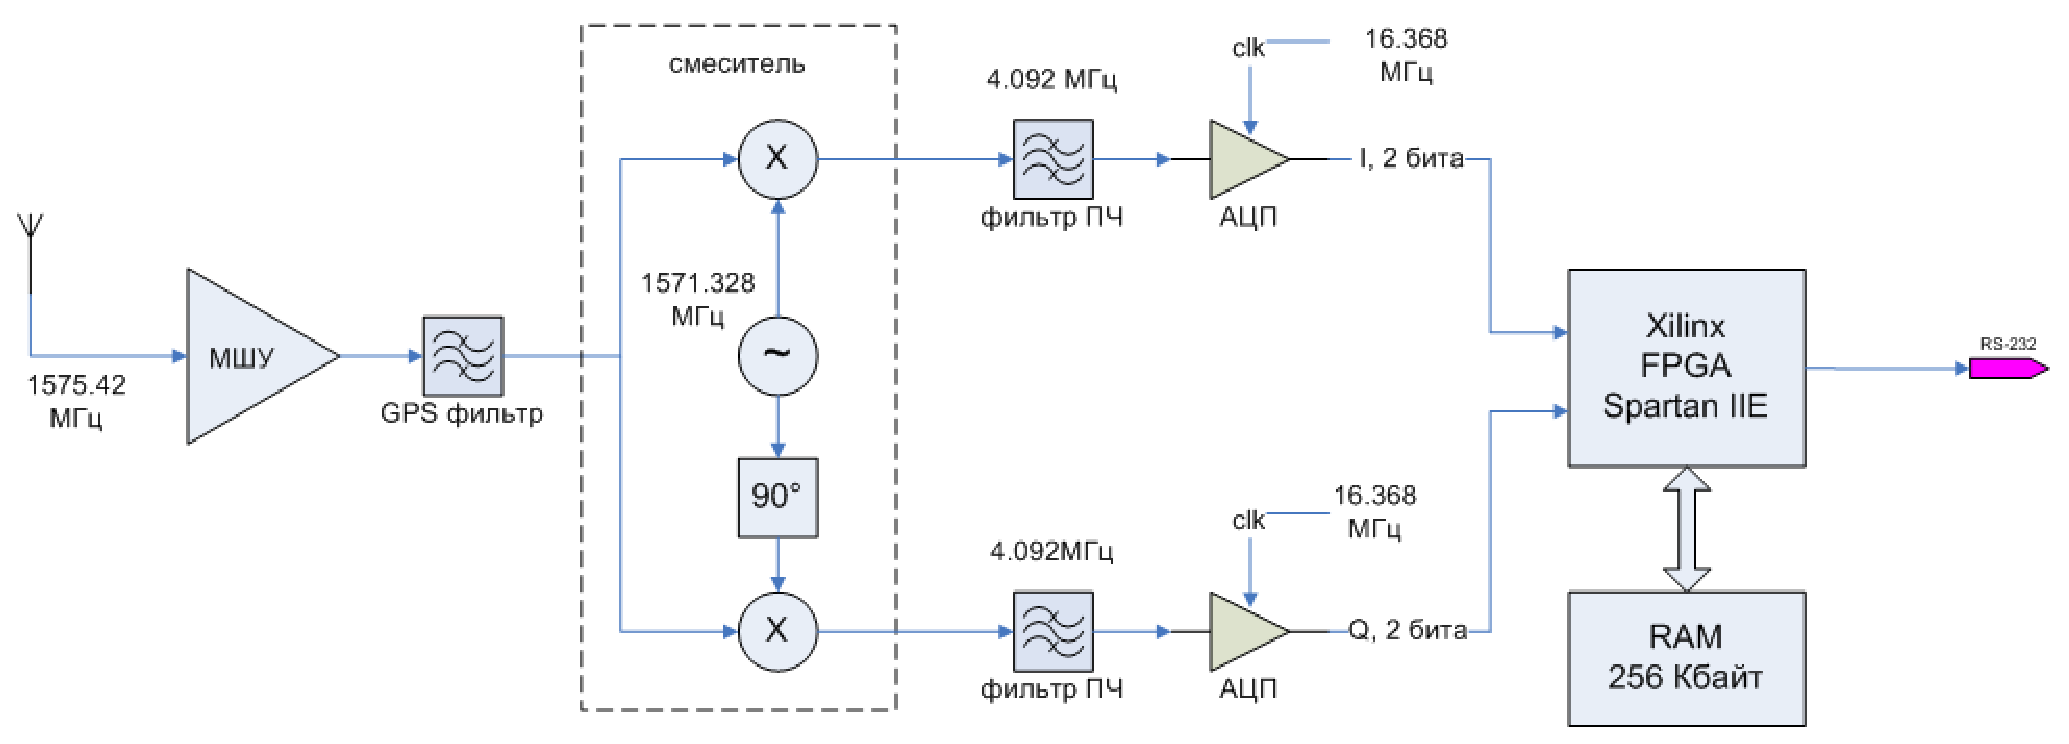
\includegraphics[width=1\linewidth]{board_scheme.eps}}
	\caption{Схема аппаратного обеспечения}
	\label{pic:board_scheme}
\end{figure}

Схема системы по захвату данных представлена на Рис. \ref{pic:gps_acq_system_scheme}. Данная система работает по схеме отложенной обработки данных. Основной сервер системы захвата
выдает команду оборудованию захвата - начать накопление данных. Оборудование захвата данных переходит в режим захвата и начинает накапливание 256 КБ данных. По окончании цикла
накопления данных оборудование захвата данных отвечает о готовности данных основному серверу системы захвата и начинает передачу данных. После передачи данных основной сервер
захвата данных публикует на публичный FTP-сервер файл с данными и прилагает к нему WAAS-картинку, которая отображает положения спутников над землей. Файл с данными
и картинку WAAS может забрать с FTP-сервера клиент для последующей работы с данными на своем ПК. В качестве диплома автор также разработал SDK для работы с файлом данных
\cite{github-gpsproject}: функции загрузки данных в MATLAB, параллельный коррелятор, генератор ПСП Голда и некоторые другие функции для облегчения работы с аппаратной платформой
и данными.

\begin{figure}[h]
	\center\scalebox{1}{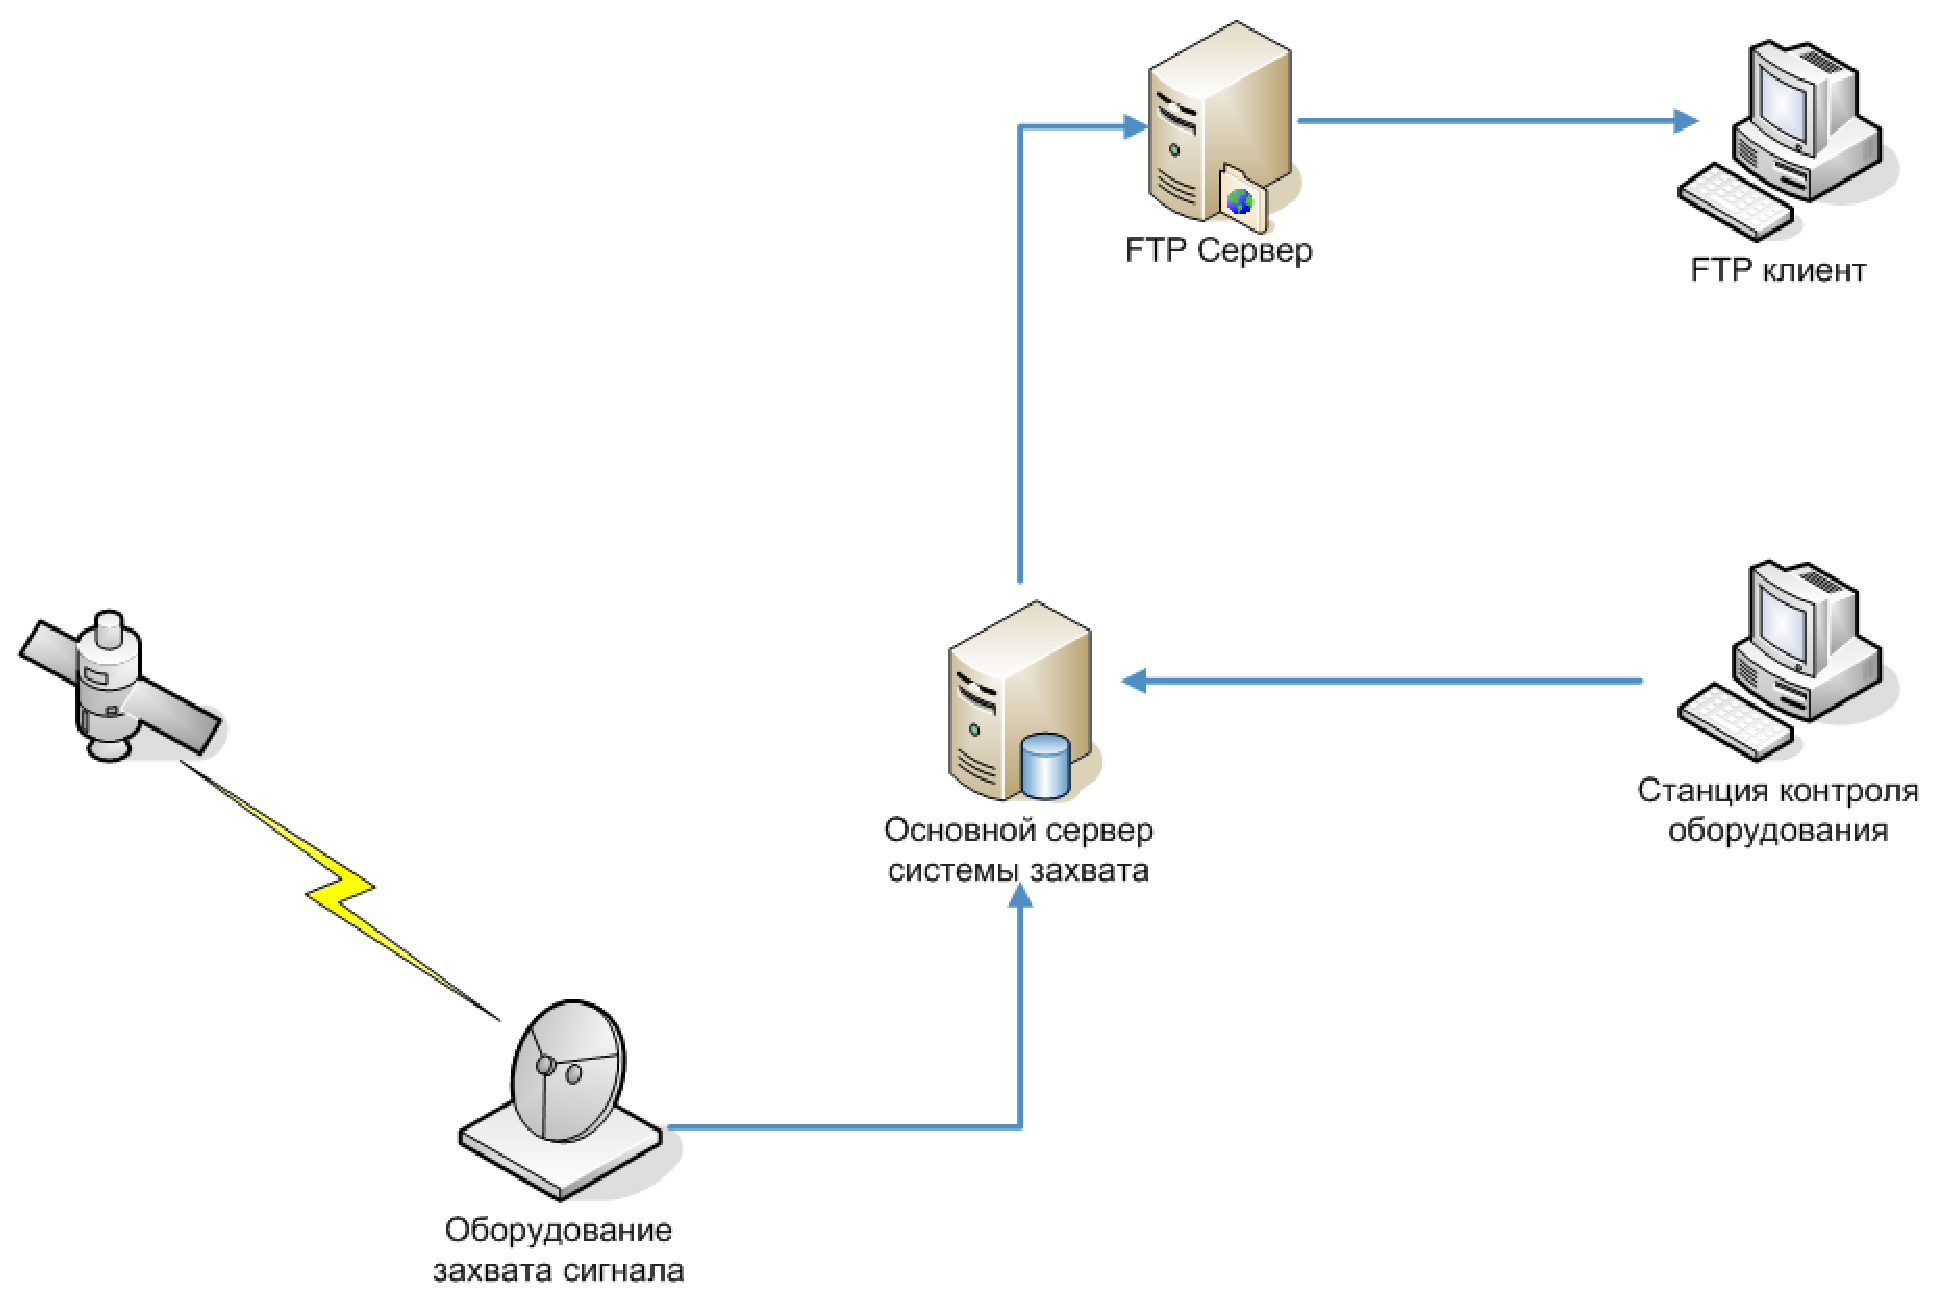
\includegraphics[width=1\linewidth]{gps_acq_system_scheme.eps}}
	\caption{Схема системы захвата данных}
	\label{pic:gps_acq_system_scheme}
\end{figure}

Структура файла с данными представлена на Рис. \ref{pic:dump_file}. В файл записываются значения управляющих регистров микросхемы MAX2769 для того, чтобы можно было
понять в каком режиме был записан файл. К доступным режимам, например, можно отнести \cite{max2769_manual}: одно- или двухквадратурный режим работы, разрядность при оцифровке
аналогового сигнала, тип захватываемых данных СНС (Глонасс, Navstar GPS, Galileo), а так же другие.
\begin{figure}[h]
	\center\scalebox{0.5}{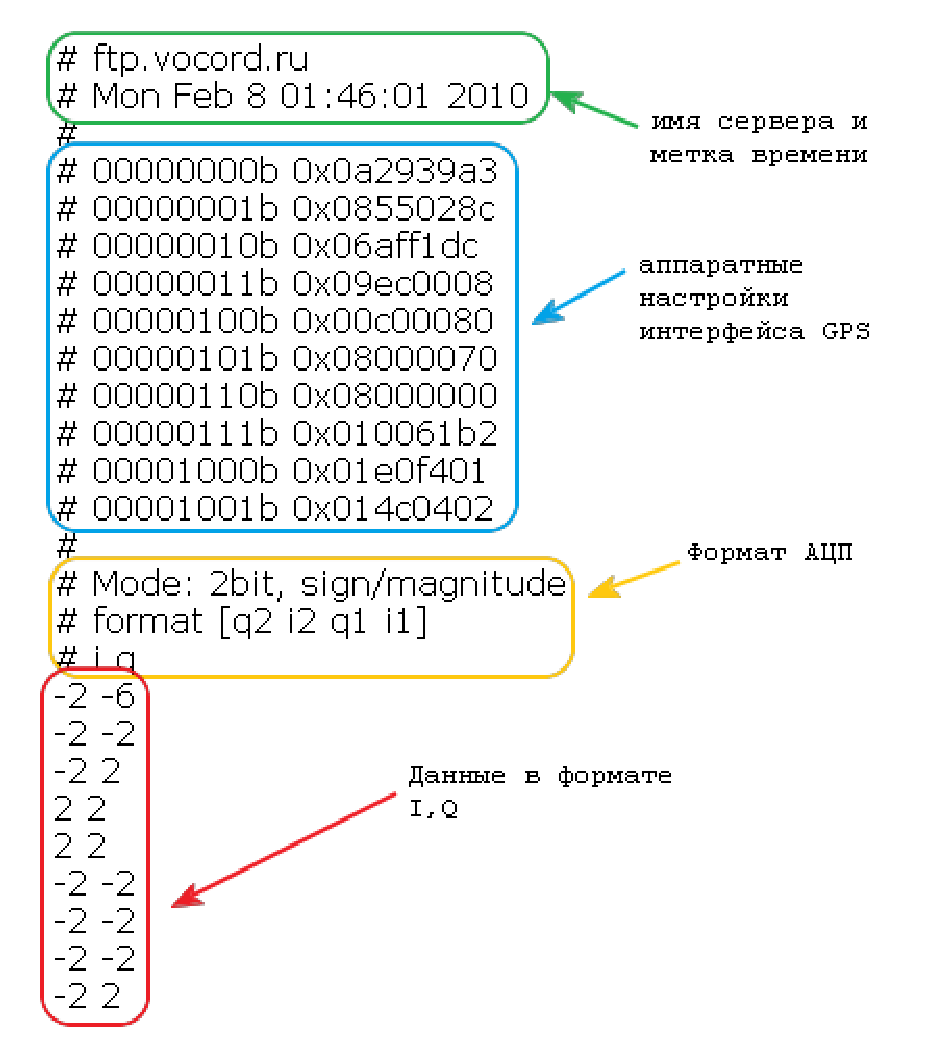
\includegraphics[width=1\linewidth]{dump_file.eps}}
	\caption{Структура файла с данными}
	\label{pic:dump_file}
\end{figure}

Полученный файл с данными оцифрован с частотой 16.368 МГц, ПЧ источников сигнала, 4.092 МГц. В качестве алгоритма оценки фазы ПСП использовался рассмотренный алгоритм DMA,
оценка частоты проводилась при помощи алгоритма основанного на применении авторегрессионной модели (АР), предложенной авторами в \cite{my_otchet}. Полученная оценка
частоты классическим коррелятором и предлагаемым алгоритмом сравнивалась (с точностью до 1 кГц), при это оценка фазы ПСП должна находиться в пределах одного чипа: ${\pm 8}$
отсчетов. При совпадении оценки фазы ПСП и оценки частоты, оценка частоты полученная предлагаемым алгоритмом подавалась на классический коррелятор для повторной проверки.

Для увеличения ОСШ в алгоритме DMA использовалось когерентное накопление сигнала. Производилось осреднение на 3 мс сигнала, что дает прирост ОСШ на 4.77 дБ.
В алгоритме на основе АР метода была взята 1 мс сигнала дополненная 3 мс нулей, для повышения спектрального разрешения при оценке АКФ посредством ДПФ.

\subsection{Результаты эксперимента}

Результат работы классического коррелятора представлены на Рис. \ref{pic:16mhz_sats_all}. Сигнал взят с 2000 отсчета, данное смещение выбрано произвольно.
\begin{figure}[h]
\center\scalebox{1}{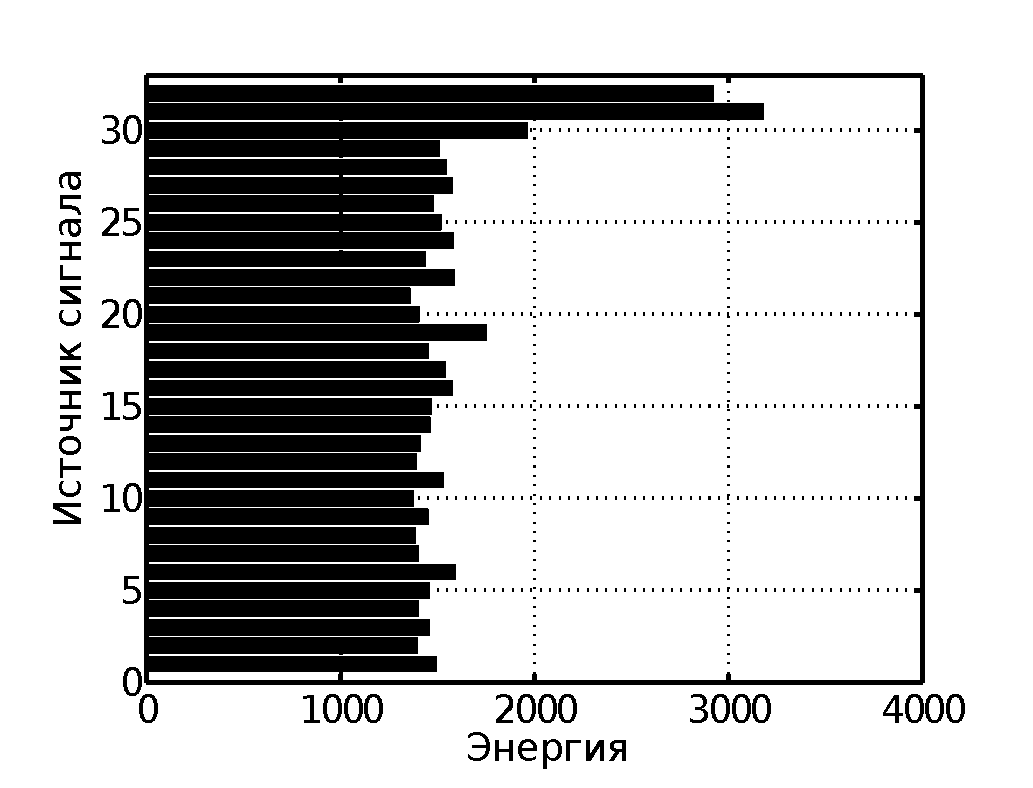
\includegraphics[width=1\linewidth]{16mhz_sats_all.eps}}
	\caption{Соотношений энергий источников сигнала}
	\label{pic:16mhz_sats_all}
\end{figure}

В виду того, что данных недостаточно для запуска модуля ФАПЧ, целесообразно рассматривать фазу ПСП и оценку частоты для сравнения работы двух
алгоритмов - таблица \ref{tbl:16mhz_sats_all} отражает данные с Рис. \ref{pic:16mhz_sats_all}.
\begin{center}
	\begin{longtable}{ | c | c | c | c |}
	\hline
	Источник сигнала & Фаза ПСП & Оценка частоты, Гц & Величина пика КФ, дБ \\ \hline
	01 & 14213	& 4091000.00	& 10.93 \\ \hline 
	02 & 4788	& 4087000.00	& 10.47 \\ \hline
	03 & 4750	& 4092000.00	& 10.59 \\ \hline
	04 & 8319	& 4097000.00	& 10.43 \\ \hline
	05 & 14143	& 4091000.00	& 10.75 \\ \hline
	06 & 7270	& 4089000.00	& 11.47 \\ \hline
	07 & 7829	& 4088000.00	& 10.46 \\ \hline
	08 & 1988	& 4092000.00	& 10.45 \\ \hline
	09 & 3571	& 4094000.00	& 10.53 \\ \hline
	10 & 2872	& 4093000.00	& 10.35 \\ \hline
	11 & 1353	& 4089000.00	& 11.09 \\ \hline
	12 & 13042	& 4097000.00	& 10.39 \\ \hline
	13 & 16311	& 4096000.00	& 10.49 \\ \hline
	14 & 11158	& 4092000.00	& 10.79 \\ \hline
	15 & 5297	& 4089000.00	& 10.86 \\ \hline
	16 & 14905	& 4094000.00	& 11.41 \\ \hline
	17 & 10017	& 4093000.00	& 11.29 \\ \hline
	18 & 11500	& 4087000.00	& 10.61 \\ \hline
	19 & 14434	& 4088000.00	& 12.57 \\ \hline
	20 & 14026	& 4094000.00	& 10.33 \\ \hline
	21 & 13463	& 4087000.00	& 10.25 \\ \hline
	22 & 2251	& 4094000.00	& 11.64 \\ \hline
	23 & 15352	& 4091000.00	& 10.55 \\ \hline
	24 & 14627	& 4094000.00	& 11.55 \\ \hline
	25 & 9910	& 4093000.00	& 11.10 \\ \hline
	26 & 934	& 4087000.00	& 10.73 \\ \hline
	27 & 8090	& 4091000.00	& 11.28 \\ \hline
	28 & 13998	& 4090000.00	& 11.29 \\ \hline
	29 & 6503	& 4087000.00	& 10.99 \\ \hline
	30 & 13592	& 4094000.00	& 12.87 \\ \hline
	31 & 4505	& 4092000.00	& 15.57 \\ \hline
	32 & 10210	& 4092000.00	& 15.50 \\ \hline
	\caption{Соотношений энергий источников сигнала}
	\label{tbl:16mhz_sats_all}
	\end{longtable}
\end{center}

Рассмотрим источники сигнала с номерами 31 и 32 как наиболее сильные.

Рассмотрим источник сигнала 31. Сравнение полученных оценок представлено в таблице \ref{tbl:16mhz_sat_31}. Оценки, полученные с использованием
предлагаемого подхода согласуются с результатами, полученными классическим подходом.
\begin{center}
	\begin{longtable}{ | c | c | c | c |}
	\hline
	Алгоритм	& Оценка фазы ПСП & Оценка частоты, Гц & Величина пика КФ, дБ \\ \hline
	АР + DMA	& 4503 & 4092277.39	& 15.60 \\ \hline
	Коррелятор & 4505 & 4092000.00	& 15.57 \\ \hline
	\caption{Оценка параметров источника сигнала 31}
	\label{tbl:16mhz_sat_31}
	\end{longtable}
\end{center}

Так же рассмотрим источник сигнала 32.  Сравнение полученных оценок представлено в таблице \ref{tbl:16mhz_sat_32}. Оценки, полученные с использованием
предлагаемого подхода согласуются с результатами, полученными классическим подходом.
\begin{center}
	\begin{longtable}{ | c | c | c | c |}
	\hline
	Алгоритм	& Оценка фазы ПСП & Оценка частоты, Гц & Величина пика КФ, дБ \\ \hline
	АР + DMA	& 10210 & 4091937.35	& 15.56 \\ \hline
	Коррелятор	& 10209 & 4092000.00   	& 15.50 \\ \hline
	\caption{Оценка параметров источника сигнала 32}
	\label{tbl:16mhz_sat_32}
	\end{longtable}
\end{center}

Из таблиц \ref{tbl:16mhz_sat_31} и \ref{tbl:16mhz_sat_32} видно, что применение предлагаемого подхода позволяет получить более точные оценки частоты. Данные
результаты согласуются с известными результатами.

%%%%%%
%\clearpage
\section{Эксперимент на данных Мишеля Боваро}

Так же полунатурное моделирование проводилось с данными собранными итальянским ученым Мишелем Боваро (Michele Bavaro) \cite{bovaro_blog}. Представленный файл с данными оцифрован
с частотой 5.456 МГц, промежуточная частота источников сигнала, 4.092 МГц. Длинна записанных данных позволяет так же проверить
вхождение системы в синхронизм. Файл больше недоступен по ссылке, приведенной в блоге Мишеля Боваро, автор представляет его по адресу \cite{rflab_primo}.
Объема данных достаточно для оценки информационных параметров и проверки вхождения с синхронизм. По этой причине в данной диссертационной работе будет
рассмотрена система ФАП, оптимальная для приема 2-ФМ манипулированного сигнала.

%%%
\subsection{Схема Костаса}

При использовании схемы Костаса осуществляется демодуляция 2-ФМ сигналов, при этом используется фазовая автоматическая подстройка (ФАП) частоты. Схема
Костаса является оптимальной \cite{shahtarin-wiener-kalman}.

В основе оптимальной нелинейной фильтрации лежит уравнение Р.Л. Стратоновича. Так как уравнение Стратоновича в общем виде решению не поддается, необходимо
перейти к системе двух уравнений:
\begin{itemize}
	\item дифференциальное уравнение относительно оцениваемых параметров;
	\item дифференциальное уравнение относительно дисперсии ошибки.
\end{itemize}

Так как приведенные уравнения являются нелинейными, при их составлении необходимо задать функцию Стратановича.

Входная смесь, содержащая 2-ФМ сигнал, может быть представлена в виде:
\begin{equation}
	x(t) = s(t, \varphi, \alpha) + n(t) = A \cos \left[ \omega_0t + \varphi(t) +\alpha \pi \right] + n(t),
	\label{eq:sec4_sig}
\end{equation}
где ${n(t)}$ - АБГШ, ${\alpha}$ принимает дискретные значения 1 или 0, амплитуда ${A}$ и частота ${\omega}$ постоянны.

Уравнения фильтрации имеют вид:
\begin{eqnarray}
	\frac{d \hat{\varphi}}{dt} = \sigma_{\hat{\varphi}}^2(p_1 F_{1}' + p_2 F_{2}'), \nonumber \\
	\frac{d \sigma_{\hat{\varphi}}^2}{dt} = \frac{1}{2}N_{\varphi} + \sigma_{\hat{\varphi}}^4(p_1 F_{1}'' + p_2 F_{2}''),
	\label{eq:sec4_filter_eq}
\end{eqnarray}
где ${p_1, p_2}$ - апостериорные вероятности состояния параметра ${\alpha}$, ${\hat{\varphi}}$ - оценка параметра ${\varphi}$, а ${\sigma_{\hat{\varphi}}^2}$ - 
дисперсия параметра ${\hat{\varphi}}$, ${N_{\varphi}}$ - односторонний энергетический спектр, ${F_i(t, \varphi)}$ - функция Стратоновича.
\begin{equation}
	F_i(t, \varphi) = \frac{2}{N_0} x(t)s(t, \varphi, \alpha_i),
	\label{eq:sec4_stratonovicha_eq}
\end{equation}
где ${i = 1, 2}$, а ${\alpha_1 = 0}$ и ${\alpha_2 = 1}$.

\begin{eqnarray}
	F_{i}' = \frac{\partial{F_i (t, \hat{\varphi})}}{\partial{\hat{\varphi}}}, \nonumber \\
	F_{i}'' = \frac{\partial^2{F_i (t, \hat{\varphi})}}{\partial{\hat{\varphi}^2}}.
	\label{eq:sec4_stratonovicha_eq_der}
\end{eqnarray}

Дифференциальные уравнение, записанные относительно  апостериорных вероятностей ${p_i}$ \cite{shahtarin-wiener-kalman}:
\begin{eqnarray}
	\frac{dp_1}{dt} = -\mu p_1 + \nu p_2 + p_1 p_2 \left[ (F_1 - F_2) + \frac{1}{2} p_1 \sigma_{\hat{\varphi}}^2 (F_1'' - F_2'') \right]; \nonumber \\
	\frac{dp_2}{dt} = \mu p_1 - \nu p_2 - p_1 p_2 \left[ (F_1 - F_2) + \frac{1}{2} p_2 \sigma_{\hat{\varphi}}^2 (F_1'' - F_2'') \right],
	\label{eq:sec4_stratonovicha_eq_der_p}
\end{eqnarray}
где ${\mu, \nu}$ - элементы матрицы интенсивностей вероятностей перехода дискретного процесса ${\alpha(t)}$:
\begin{equation}
	\label{eq:sec4_alpha}
	\{\alpha_{ij}\}
	=
		\left[ \begin{array}{cc}
			-\mu	&	\mu \\
			\nu 	&	-\nu
		\end{array} \right],
\end{equation}
где ${i,j = 1,2}$.

Принятие решения о значении параметра ${\alpha}$ возможно по значению знака разности апостериорных вероятностей ${z = p_1 - p_2}$. В данном случае
при учете соотношений:
\begin{eqnarray}
	p_1 + p_2 = 1; \nonumber \\
	p_1 = \frac{1+z}{2}; \nonumber \\
	p_2 = \frac{1-z}{2}.
	\label{eq:sec4_probability}
\end{eqnarray}

Количество уравнений системы может быть сокращено до трех:
\begin{eqnarray}
	\frac{d \hat{\varphi}}{dt} & = & \frac{1}{2}\sigma_{\hat{\varphi}}^2 \left[(F_{1}' + F_{2}') + z(F_{1}' - F_{2}') \right]; \nonumber \\
	\frac{d \sigma_{\hat{\varphi}}^2}{dt} & = & \frac{1}{2}N_{\varphi} + \frac{1}{2}\sigma_{\hat{\varphi}}^4 \left[ (F_{1}'' + F_{2}'') +  z(F_{1}'' - F_{2}'') \right]; \\
	\frac{dz}{dt} & = & (\nu - \mu) - (\nu + \mu)z + \frac{1}{2}(1 - z^2) \left[ (F_{1} - F_{2}) +  \frac{1}{2} \sigma_{\hat{\varphi}}^2 (F_{1}'' - F_{2}'') \right]. \nonumber
	\label{eq:sec4_stratonovich_3}
\end{eqnarray}

В случае когда принимаемый сигнал модулирован оп закону 2-ФМ, когда параметра ${\alpha}$ принимает два дискретных значения 0 и 1,
функция Стратоновича записывается как \cite{shahtarin-wiener-kalman}:
\begin{equation}
	F_1(t, \varphi) = \frac{2A}{N_0}x(t) \cos (\omega_0 t + \varphi) = -F_2(t, \varphi)
	\label{eq:sec4_stratonovich_bpsk}
\end{equation}

Сигналы ${s_1(t)}$ и ${s_2(t)}$ определяются равенством: 
\begin{equation}
	s_1(t, \varphi) = -s_2(t, \varphi) = A \cos \left[ \omega_0 t \varphi(t) \right].
	\label{eq:sec4_s1_s2}
\end{equation}

В данном случае:
\begin{eqnarray}
	F_1' + F_2' & = & 0; \nonumber \\
	F_1'' + F_2'' & = & 0; \nonumber \\
	F_1 - F_2 & = & 2F_1 = \frac{4A}{N_0}x(t) \cos(\omega_0 t + \hat{\varphi}); \nonumber \\
	F_1' - F_2' & = & 2F_1' = -\frac{4A}{N_0}x(t) \sin(\omega_0 t + \hat{\varphi}); \nonumber \\
	F_1'' - F_2'' & = & 2F_1'' = -\frac{4A}{N_0}x(t) \cos(\omega_0 t + \hat{\varphi}) = -2F_1. \nonumber \\
	\label{eq:sec4_strat_der}
\end{eqnarray}

При ${\nu = \mu = \frac{1}{2}}$ выражения \ref{eq:sec4_stratonovich_3} принимают вид:
\begin{eqnarray}
	\frac{d \hat{\varphi}}{dt} + \frac{2A}{N_0} \sigma_{\hat{\varphi}}^2 z x(t) \sin (\omega_0 t + \hat{\varphi}) & = & 0; \nonumber \\
	\frac{d \hat{\varphi}^2}{dt} = \frac{1}{2} N_{\varphi} - \sigma_{\hat{\varphi}}^4 z \frac{2A}{N_0} x(t) \cos(\omega_0 t + \hat{\varphi}) & = & \frac{1}{2}N_{\varphi} - \sigma_{\hat{\varphi}}^4 zF_1(t, \hat{\varphi}); \nonumber \\
	\frac{dz}{dt} = -z + (1 - z^2) \left( 1 - \frac{1}{2} \sigma_{\hat{\varphi}}^2 \right) x(t) \cos(\omega_0 t + \hat{\varphi}) & = & \nonumber \\
		 = -z + (1 - z^2) \left( 1 - \frac{1}{2} \sigma_{\hat{\varphi}}^2 \right) F_1(t, \hat{\varphi}), & &
	\label{eq:sec4_strat_der111}
\end{eqnarray}
в тоже время ${1 - z^2 \ge 0}$.


В случае ${z=th \int_{t_k}^t F_1(t, \hat{\varphi}) d\varphi}$ схема алгоритма соответствует оптимальному приемнику, по критерию МАВ \cite{shahtarin-wiener-kalman}, а при ${thx \approx x}$
соответствует схеме Костаса.

%\begin{figure}[h]
%\center\scalebox{1}{\includegraphics[width=1\linewidth]{costas_loop.eps}}
%	\caption{Схема Костаса}
%	\label{pic:sec4_costas
%\end{figure}
`
%%%
В качестве алгоритма оценки фазы ПСП использовался
рассмотренный алгоритм DMA, оценка частоты проводилась при помощи алгоритма основанного на применении авторегрессионной модели (АР).
Полученная оценка подавалась на модуль фазовой автоподстройки частоты (ФАПЧ) и проверялось вхождение в синхронизм.

Для увеличения ОСШ в алгоритме DMA использовалось когерентное накопление сигнала. Производилось осреднение на 3 мс сигнала, что дает прирост ОСШ на 4.77 дБ.
В алгоритме на основе АР метода была взята 1 мс сигнала дополненная 3 мс нулей, для повышения спектрального разрешения при оценке АКФ посредством ДПФ.

В качестве модуля ФАПЧ взят код американского ученого Дениса Акоса (Dennis M. Akos) \cite{sandiaproject}.
Параметры выбранные для ФАПЧ: коэффициент демпфирования ${\zeta=0.7}$, шумовая полоса  ${B_L=40}$ Гц. 

\subsection{Результаты эксперимента}

Результат работы классического коррелятора представлены на Рис. \ref{pic:5mhz_sats_all}. Сигнал взят с 2000 отсчета, данное смещение выбрано произвольно.
\begin{figure}[h]
\center\scalebox{1}{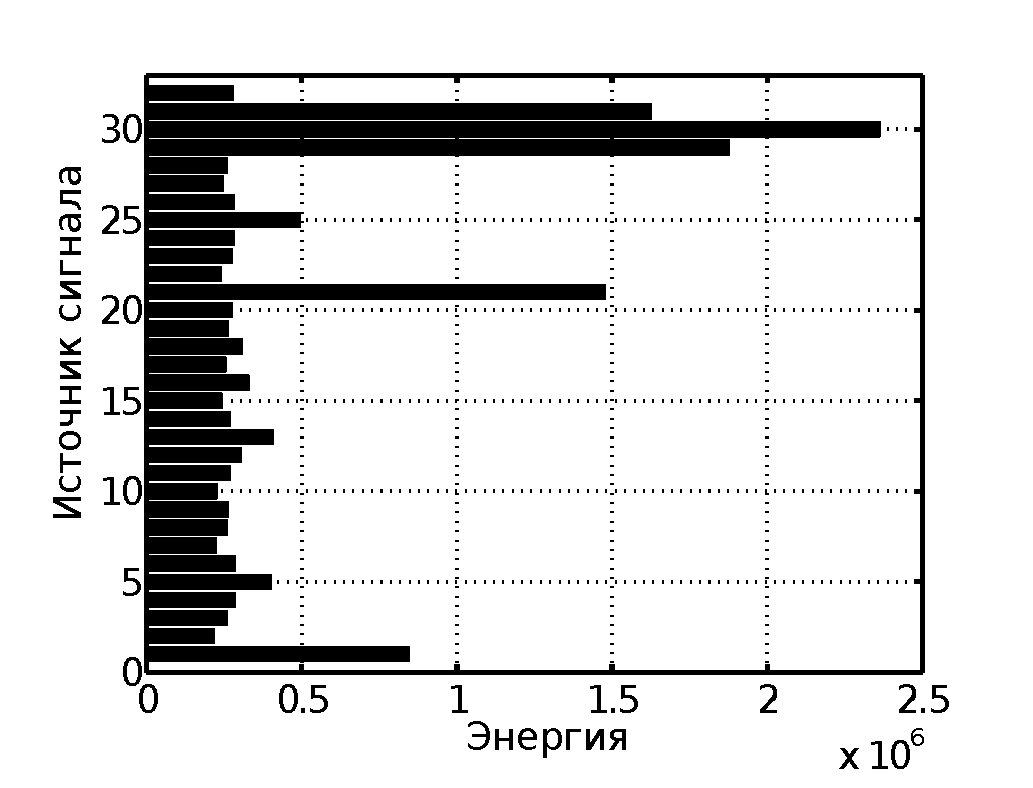
\includegraphics[width=1\linewidth]{5mhz_sats_all.eps}}
	\caption{Соотношений энергий источников сигнала}
	\label{pic:5mhz_sats_all}
\end{figure}

В таблице \ref{tbl:5mhz_sats_all} представлены оценки фаз ПСП и частот для Рис. \ref{pic:5mhz_sats_all}.
\begin{center}
	\begin{longtable}{ | c | c | c | c |}
	\hline
	Источник сигнала & Фаза ПСП & Оценка частоты, Гц & Величина пика КФ, дБ \\ \hline
	01 & 3056 & 4093000.00 & 14.64 \\ \hline 
	02 & 776  & 4090000.00 & 9.79  \\ \hline
	03 & 2372 & 4087000.00 & 10.33 \\ \hline
	04 & 1951 & 4089000.00 & 10.79 \\ \hline
	05 & 1231 & 4093000.00 & 12.11 \\ \hline
	06 & 3565 & 4087000.00 & 10.72 \\ \hline
	07 & 4576 & 4091000.00 & 9.79  \\ \hline
	08 & 1177 & 4097000.00 & 10.25 \\ \hline
	09 & 4665 & 4090000.00 & 10.08 \\ \hline
	10 & 387  & 4088000.00 & 10.03 \\ \hline
	11 & 3805 & 4095000.00 & 10.74 \\ \hline
	12 & 762  & 4094000.00 & 11.00 \\ \hline
	13 & 1027 & 4093000.00 & 12.35 \\ \hline
	14 & 1504 & 4090000.00 & 10.50 \\ \hline
	15 & 4885 & 4088000.00 & 10.05 \\ \hline
	16 & 3700 & 4094000.00 & 11.39 \\ \hline
	17 & 3509 & 4093000.00 & 10.40 \\ \hline
	18 & 219  & 4095000.00 & 11.35 \\ \hline
	19 & 4731 & 4088000.00 & 10.57 \\ \hline
	20 & 1893 & 4093000.00 & 10.67 \\ \hline
	21 & 1677 & 4094000.00 & 15.60 \\ \hline
	22 & 2949 & 4091000.00 & 10.36 \\ \hline
	23 & 2268 & 4091000.00 & 10.75 \\ \hline
	24 & 4090 & 4090000.00 & 11.00 \\ \hline
	25 & 4324 & 4088000.00 & 12.97 \\ \hline
	26 & 3572 & 4090000.00 & 10.69 \\ \hline
	27 & 3372 & 4092000.00 & 10.26 \\ \hline
	28 & 4462 & 4088000.00 & 10.16 \\ \hline
	29 & 2212 & 4090000.00 & 16.00 \\ \hline
	30 & 1118 & 4090000.00 & 16.13 \\ \hline
	31 & 4850 & 4090000.00 & 15.91 \\ \hline
	32 & 4609 & 4095000.00 & 10.58 \\ \hline
	\caption{Соотношений энергий источников сигнала}
	\label{tbl:5mhz_sats_all}
	\end{longtable}
\end{center}

Рассмотрим источник сигнала 1 – Рис. \ref{pic:5mhz_sat_1}. Оценка частоты полученная параллельным коррелятором – 4.093 МГц,
оценка полученная алгоритмом на основе АР метода – 4093378.19 МГц. Видно, что система вошла в синхронизм и данные могут быть успешно демодулированы.
\begin{figure}[h]
\center\scalebox{1}{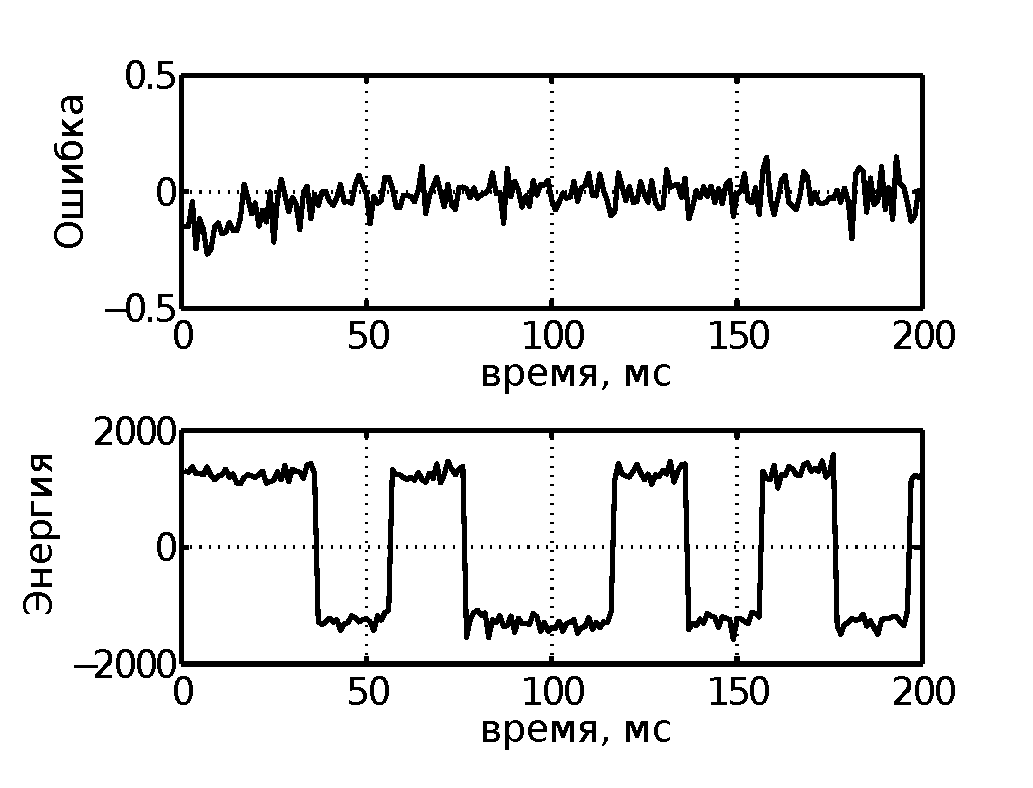
\includegraphics[width=1\linewidth]{5mhz_sat_1.eps}}
	\caption{Спутник 1}
	\label{pic:5mhz_sat_1}
\end{figure}

Рассмотрим источник сигнала 29 – Рис. \ref{pic:5mhz_sat_29}. Оценка частоты полученная параллельным коррелятором – 4.090 МГц,
оценка полученная алгоритмом на основе АР метода – 4089793.94 МГц. Видно, что система вошла в синхронизм и данные могут быть успешно демодулированы.
\begin{figure}[h]
\center\scalebox{1}{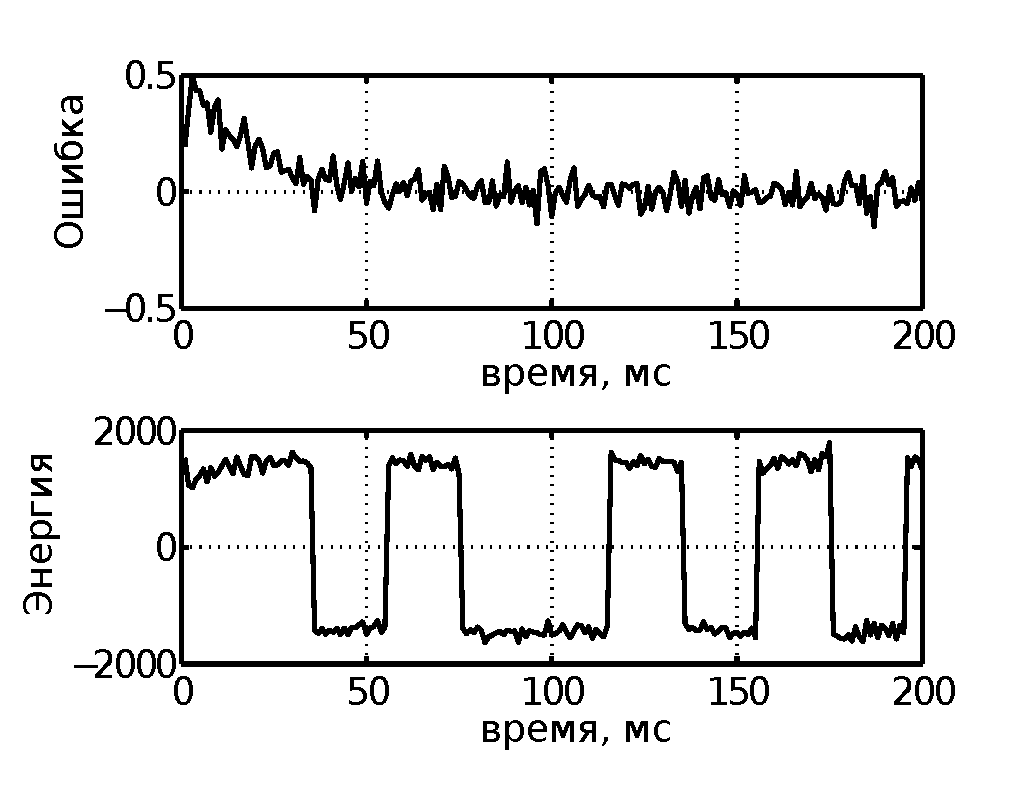
\includegraphics[width=1\linewidth]{5mhz_sat_29.eps}}
	\caption{Спутник 29}
	\label{pic:5mhz_sat_29}
\end{figure}

Рассмотрим источник сигнала 30 – Рис. \ref{pic:5mhz_sat_30}. Оценка частоты полученная параллельным коррелятором – 4.090 МГц,
оценка полученная алгоритмом на основе АР метода – 4089848.47 МГц. Видно, что система вошла в синхронизм и данные могут быть успешно демодулированы.
\begin{figure}[h]
\center\scalebox{1}{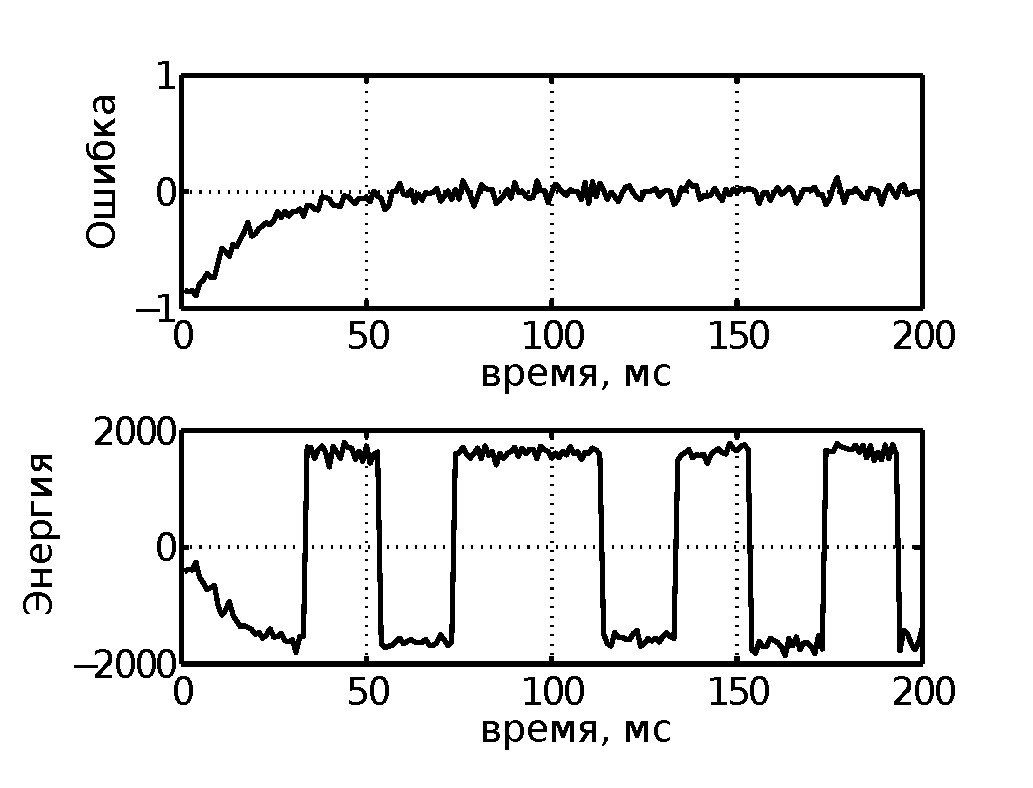
\includegraphics[width=1\linewidth]{5mhz_sat_30.eps}}
	\caption{Спутник 30}
	\label{pic:5mhz_sat_30}
\end{figure}

Рассмотрим источник сигнала 31 – Рис. \ref{pic:5mhz_sat_31}. Оценка частоты полученная параллельным коррелятором – 4.090 МГц,
оценка полученная алгоритмом на основе АР метода – 4090079.16 МГц. Видно, что система вошла в синхронизм и данные также могут быть успешно демодулированы.
\begin{figure}[h]
\center\scalebox{1}{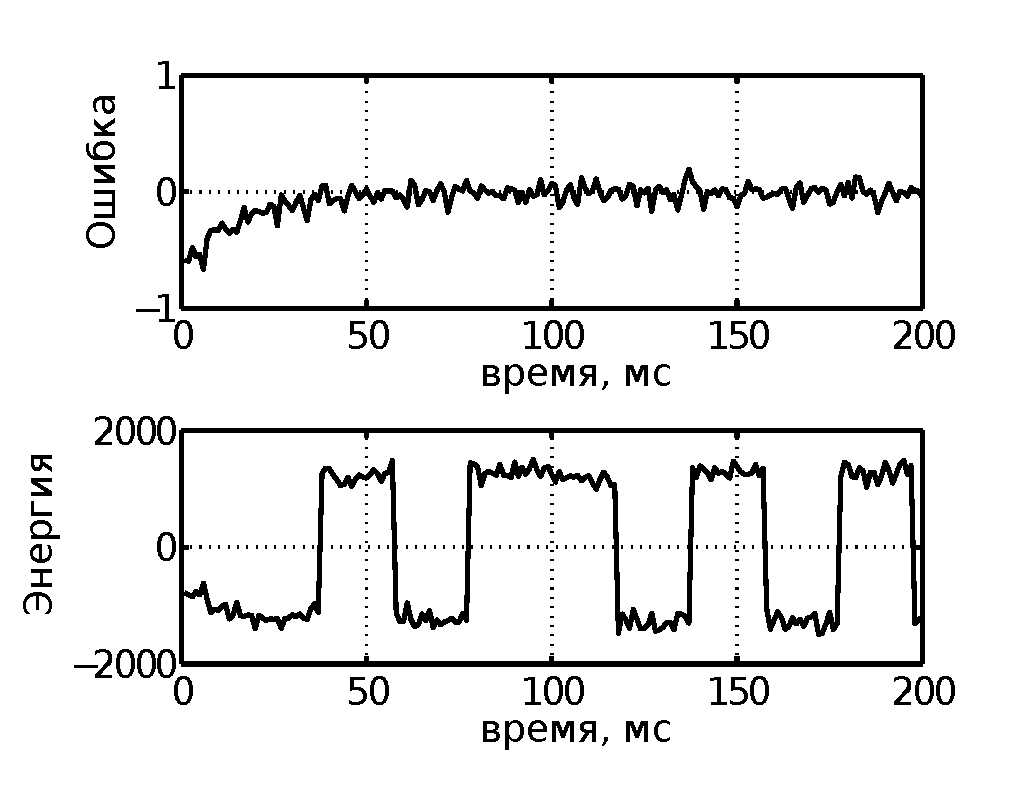
\includegraphics[width=1\linewidth]{5mhz_sat_31.eps}}
	\caption{Спутник 31}
	\label{pic:5mhz_sat_31}
\end{figure}

В то же время, параметры сигнала спутника 21, который тоже имеет достаточно высокую энергию, не смогли быть оценены - Рис. \ref{pic:5mhz_sat_21}.
\begin{figure}[h]
\center\scalebox{1}{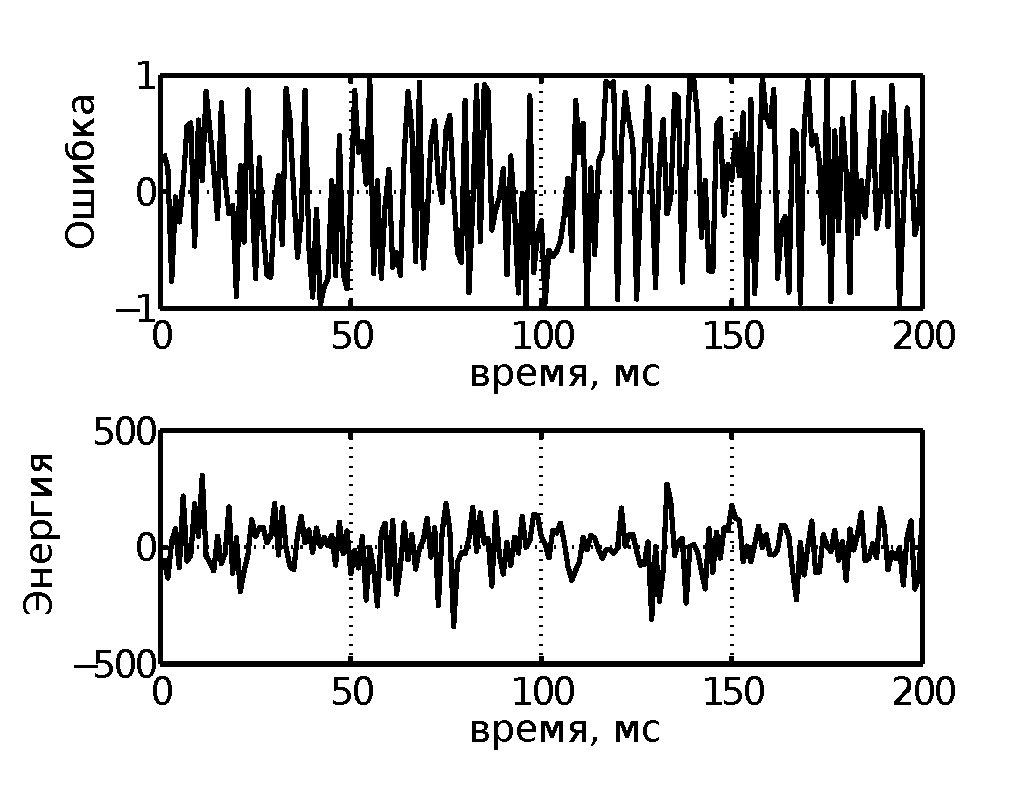
\includegraphics[width=1\linewidth]{5mhz_sat_21.eps}}
	\caption{Спутник 21}
	\label{pic:5mhz_sat_21}
\end{figure}

\begin{itemize}
\item Использование алгоритма Delay and Multiply Approach позволяет свести поиск в двумерной области неопределенности: частота и фаза к поиску только в области частоты. 
\item Применение усовершенствованного итеративного алгоритма вычисления АКФ позволяет существенно улучшить ОСШ при оценке АКФ.
\item Применение АР(2) для оценки частоты одного источника позволяет получать более точные оценки в сравнении с типовым алгоритмом.
\end{itemize}

\clearpage

\chapter*{Основные результаты и выводы}
\addcontentsline{toc}{chapter}{Основные результаты и выводы}

В итоге проведенных в диссертационной работе теоретических и экспериментальных исследований получены следующие основные результаты:
\begin{enumerate}
	\item Разработан алгоритм на основе параметрического метода оценки информационных для одного источника с CDMA-сигналом на фоне аддитивного белого гауссового шума при отстутствии МКИ.
		Получены значение вычислительной сложности и точности оценки частоты. Алгоритм на основе праметрического метода оценки частоты позволяет снизить вычислительные
		затраты в 1.5 раза в сравнении с типовым подходом при этом точность оценки, при отсутствии МКИ, не привосходит нескольких десятков герц для сигналов
		с ОСШ более 25 дБ.
	\item Усовершенствован алгоритм итеративного вычисления автокорреляционной функции. Получены значение вычислительной сложности и оценка
		прироста ОСШ в зависимости от количества итераций. Алгоритм позволяет увеличить ОСШ на 20 дБ при вычислении трех итераций
		пересчета автокорреляционной функции, в то же время вычислительная сложность, сниженная с квадратичной до логарифмической,
		позволяет использовать его в приемниках реального времени.
	\item Разработан комплексированный алгоритм оценки информационных параметров CDMA-сигнала на основе алгоритма Delay and Multiply Approach с использованием
		предложенного усовершенствованного итеративного алгоритма вычисления автокорреляционной функции и параметрического
		метода оценки частоты на фоне аддитивного белого гауссового шума при наличии МКИ. Алгоритм позволяет получить оценку частоты, удовлетворяющую
		допустимой входной расстройке ФАПЧ, для значений ОСШ сигнала порядка -20 дБ без накопления, при вычислительной сложности в 3 раза меньшей в сравнении с традиционным подходом.
	\item Результаты исследований с использованием имитационного моделирования в математическом пакете MATLAB, а также полунатурного моделирования,
		на разработанной программно-аппаратной платформе и сигнале, полученном из внешних источников, согласуются и подтверждают возможность
		использования разработанного комплексированного алгоритма оценки информационных параметров CDMA-сигнала в системе Navstar GPS у уровнем ОСШ порядка -27 дБ.
	\item Предложенный комплексированный алгоритм оценки информационных параметров CDMA-сигнала позволяет добиться наилучших результатов при
		типовых значениях допплеровского смещения и типовых сценариях распространения сигнала в наземных пользовательских приемниках.
\end{enumerate}


\clearpage
